%% fichier sys_dig.tex
%%%%%%%%%%%%%%%%

\documentclass[a4paper, 12pt, twoside]{report}

\usepackage[utf8]{inputenc}
\usepackage[T1]{fontenc}
\usepackage[francais]{babel}
\usepackage{eurosym}
\usepackage{graphicx}
\usepackage{wrapfig}
\usepackage[bookmarks=true, bookmarksnumbered=true, linkcolor={0 0 1}, linkbordercolor={1 1 1}, pdfborderstyle={/S/U/W 1}]{hyperref}
\setcounter{tocdepth}{5}

\makeatletter
\renewcommand{\thesection}{\@arabic\c@section}
\makeatother

\usepackage{fancyhdr}
\usepackage{amsthm}
\usepackage{amsmath}
\usepackage{amsfonts}
\usepackage{amssymb}
\usepackage{mathrsfs}

\usepackage{enumerate}

\usepackage{color}
\definecolor{mygreen}{rgb}{0,0.6,0}
\definecolor{mygray}{rgb}{0.5,0.5,0.5}
\definecolor{mymauve}{rgb}{0.58,0,0.82}

\usepackage{listings}
\lstset{ %
  backgroundcolor=\color{white},   % choose the background color; you must add \usepackage{color} or \usepackage{xcolor}
  basicstyle=\footnotesize,        % the size of the fonts that are used for the code
  breakatwhitespace=false,         % sets if automatic breaks should only happen at whitespace
  breaklines=true,                 % sets automatic line breaking
  captionpos=b,                    % sets the caption-position to bottom
  commentstyle=\color{mygreen},    % comment style
  extendedchars=true,              % lets you use non-ASCII characters; for 8-bits encodings only, does not work with UTF-8
  frame=single,                    % adds a frame around the code
  keepspaces=true,                 % keeps spaces in text, useful for keeping indentation of code (possibly needs columns=flexible)
  keywordstyle=\color{blue},       % keyword style
  language=C,                 % the language of the code
  numbers=left,                    % where to put the line-numbers; possible values are (none, left, right)
  numbersep=5pt,                   % how far the line-numbers are from the code
  numberstyle=\tiny\color{mygray}, % the style that is used for the line-numbers
  rulecolor=\color{black},         % if not set, the frame-color may be changed on line-breaks within not-black text (e.g. comments (green here))
  showspaces=false,                % show spaces everywhere adding particular underscores; it overrides 'showstringspaces'
  showstringspaces=false,          % underline spaces within strings only
  showtabs=false,                  % show tabs within strings adding particular underscores
  stepnumber=1,                    % the step between two line-numbers. If it's 1, each line will be numbered
  stringstyle=\color{mymauve},     % string literal style
  tabsize=2,                       % sets default tabsize to 2 spaces
  title=\lstname                   % show the filename of files included with \lstinputlisting; also try caption instead of title
}


\usepackage[top=3cm, bottom=3cm, left=3cm, right=3cm]{geometry}

\lhead{Ecole Normale Supérieure}
\rhead{}
\lfoot{}
\rfoot{}
\renewcommand{\headrulewidth}{0.4pt}
\renewcommand{\footrulewidth}{0.4pt}

\newcommand{\HRule}{\rule{\linewidth}{0.5mm}}
\pagestyle{fancy}

\newtheorem{definition}{Définition}[section]
\newtheorem{proposition}{Proposition}[section]

\begin{document}
%%%%%%%%%%%%%%%%

\begin{titlepage}
\begin{center}

% Upper part of the page. The '~' is needed because \\
% only works if a paragraph has started.

\includegraphics[width=0.35\textwidth]{./ENS_Logo.png}~\\[1cm]

\textsc{\Large Système Digital}\\[0.5cm]

% Title
\HRule \\[0.4cm{ \huge \bfseries Microprocesseur \\[0.4cm] }
\large{\textit{Implémentation d'une horloge digitale}}]

\HRule \\[1.5cm]
\end{center}

% Author and supervisor
\begin{minipage}{0.4\textwidth}
\begin{flushleft} \large
\emph{Auteurs :}\\
Nicolas ASSOUAD\\
\end{flushleft}
\end{minipage}

\begin{center}
\vfill
% Bottom of the page
{\large \today}

\end{center}
\end{titlepage}

\newpage\strut
%%%%%%%%%%%%%%%%
\tableofcontents
\thispagestyle{fancyplain}

\newpage~
\newpage~
%%%%%%%%%%%%%%%%

\section*{Introduction}
\addcontentsline{toc}{section}{Introduction}

Dans le cadre du cours de Système Digital, nous sommes amenés à concevoir un microprocesseur
qui sera capable notamment d'exécuter un programme de montre électronique.
Nous allons d'abord présenter les choix de conception de notre microprocesseur
puis nous discuterons du programme de l'horloge digitale en lui même.

\newpage~
\newpage~

\section{Le Microprocesseur}

\subsection{Le concept}

Notre ligne directrice de conception de notre microprocesseur a été de n'implémenter que 
les opérations de bases en matériel, et de laisser le soin au programmeur ou à un 
éventuel compilateur de les combiner pour produire des opérations plus évoluées.
Néanmoins, le jeu d'instruction pourrait être encore plus réduit, mais cela ne jouerait 
pas en faveur des performances.

Le schéma global du microprocesseur suit ce schéma de principe (qui se précisera 
quand la Netlist sera bien finalisé en Minijazz) :\\

\begin{figure}[!h]
\centering
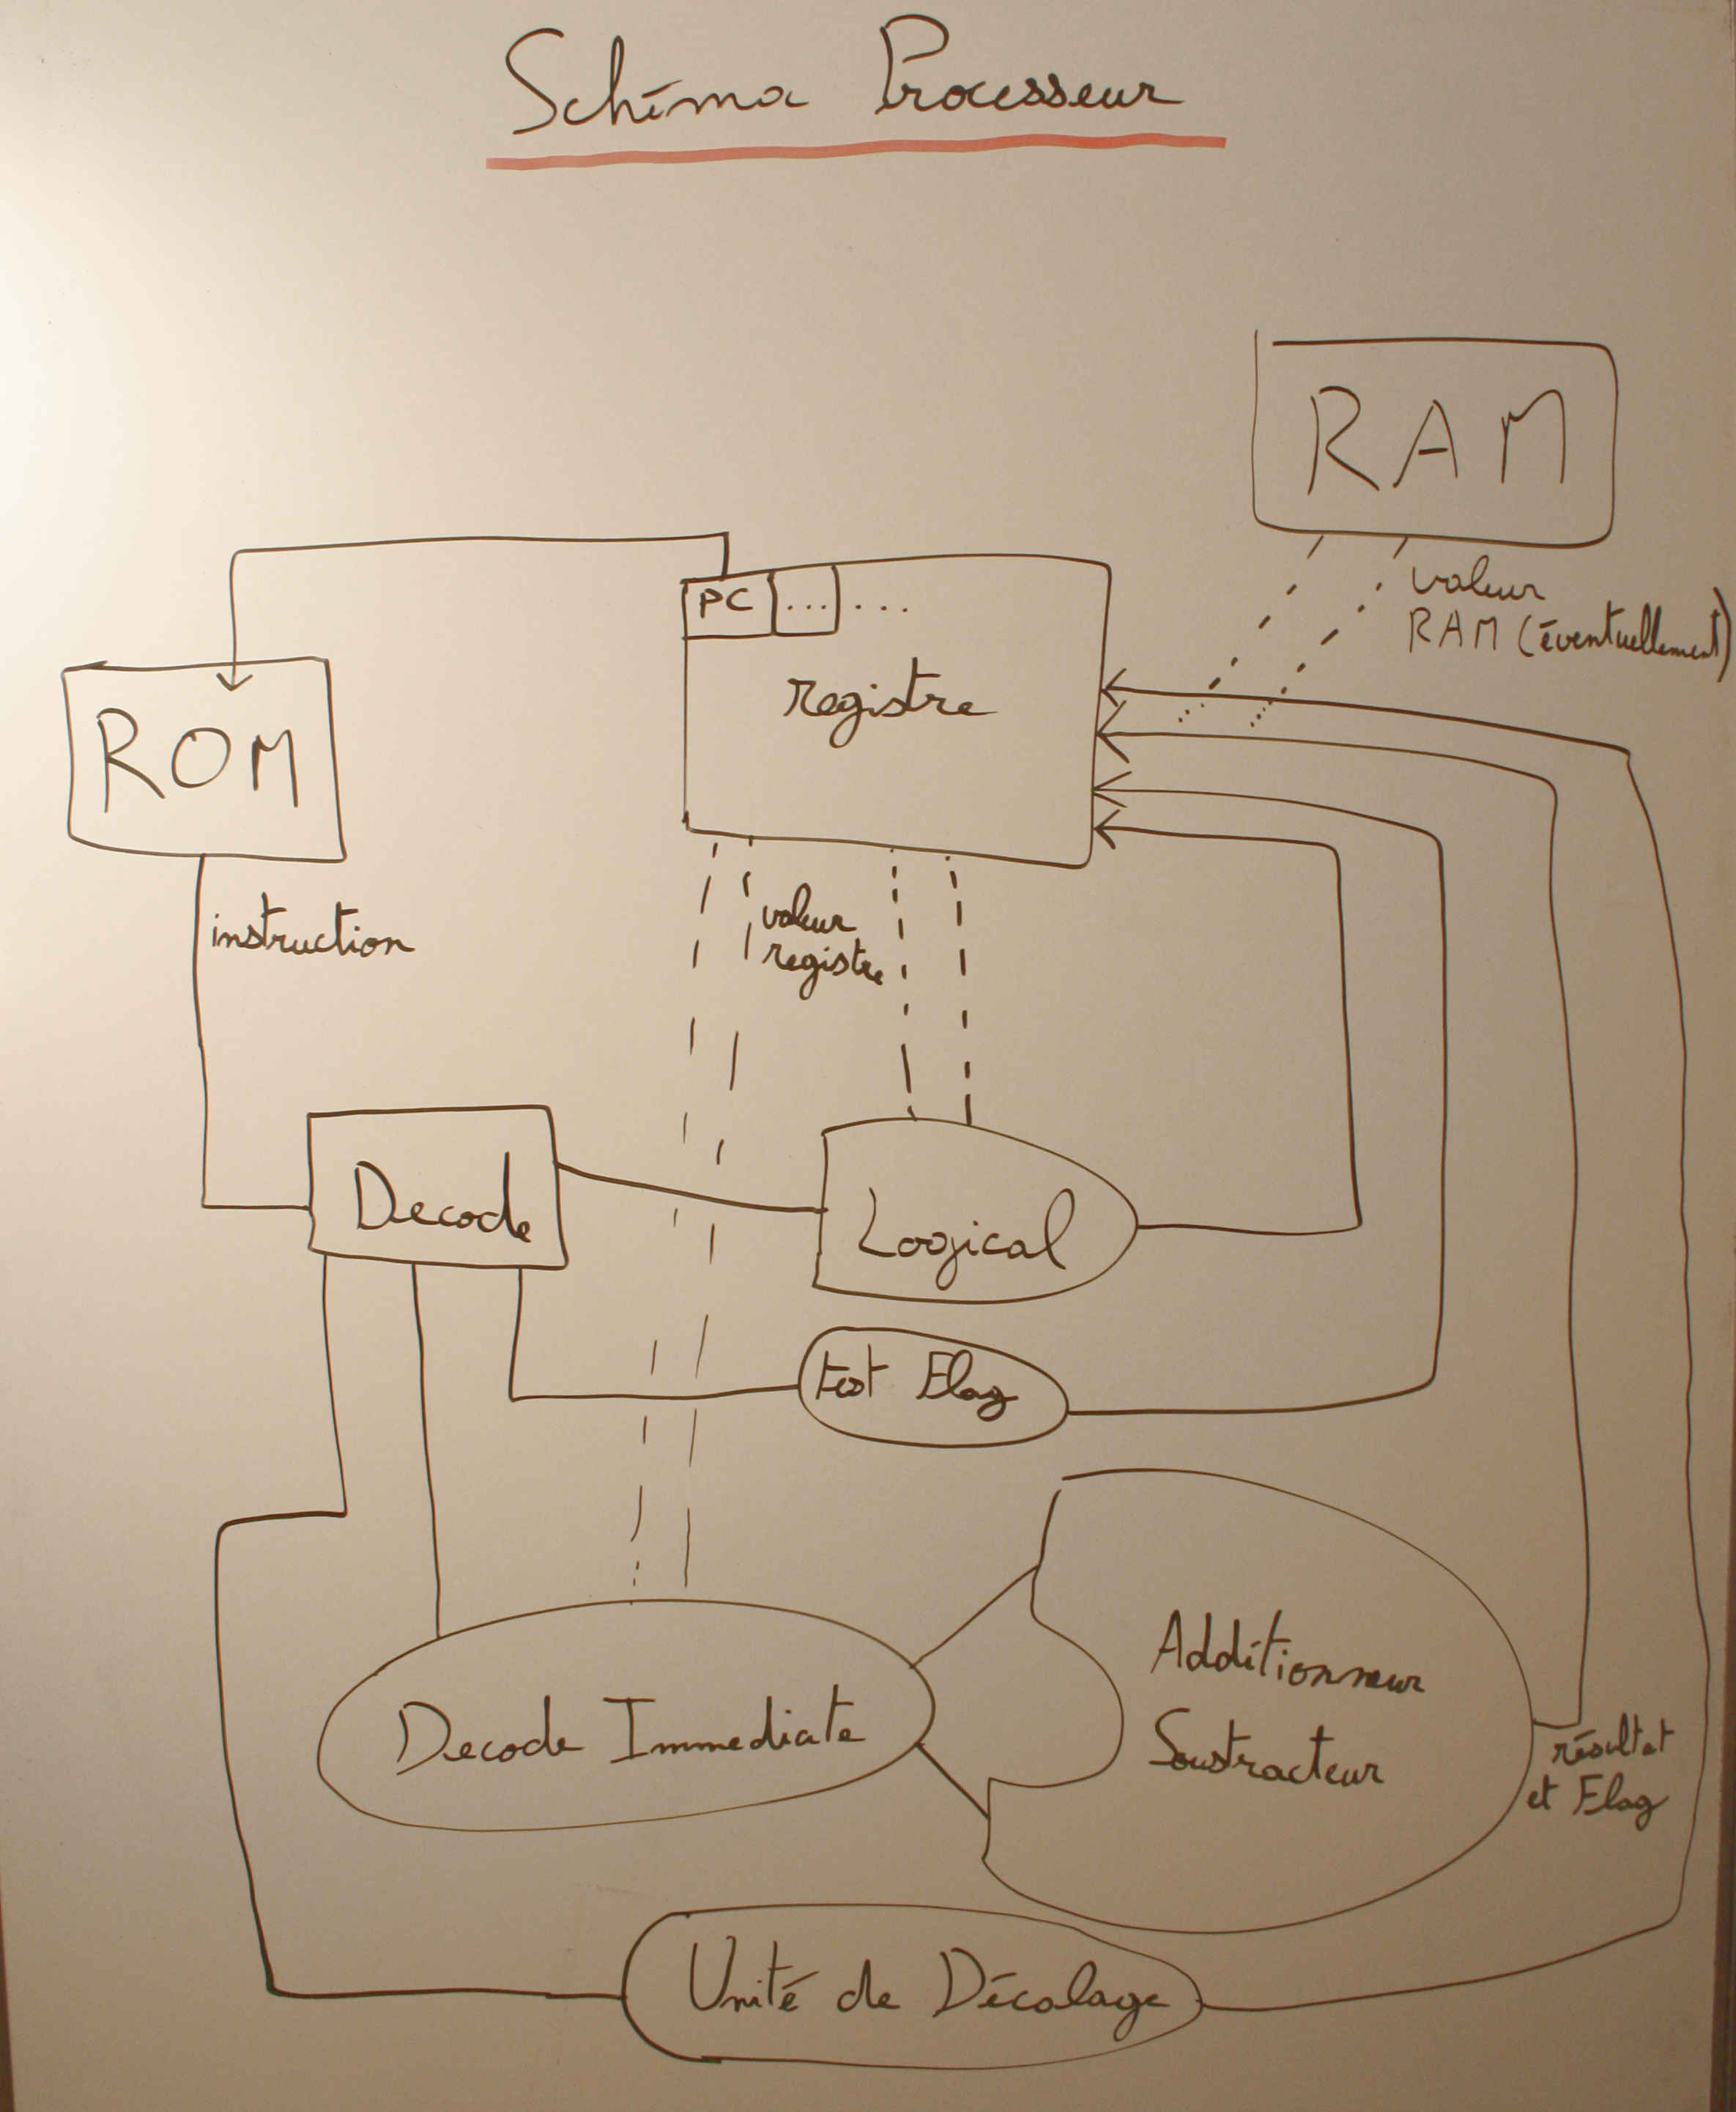
\includegraphics[width=10cm]{schema_micro.jpg}
%\caption{Cryptage Asymétrique}
\end{figure}

Le microprocesseur possède 32 registres différents dont certain spéciaux comme le 
pointeur d'instructions PC. Il sont numérotés de 1 à 30, le $31^{ieme}$ registre étant le 
registre contenant la valeur du "flag" (il prendra d'ailleurs la dénomination flag dans
le code), et le $32^{ieme}$ registre étant lui le registre du compteur d'instructions
(qui sera noté PC dans le code).

Les mots mémoires sont des mots de 32 bits, si bien que toutes les opérations matérielles
se font sur des entiers signés de 32 bits (à cela, il faut noter l'exception des calculs 
avec des valeurs immédiates dans les instructions qui, elles, sont représentées sur 
16 bits). Cela donne une implémentation de l'additionneur/soustracteur que le peut
représenter de la manière suivante par un schéma :\\

\begin{figure}[!h]
\centering
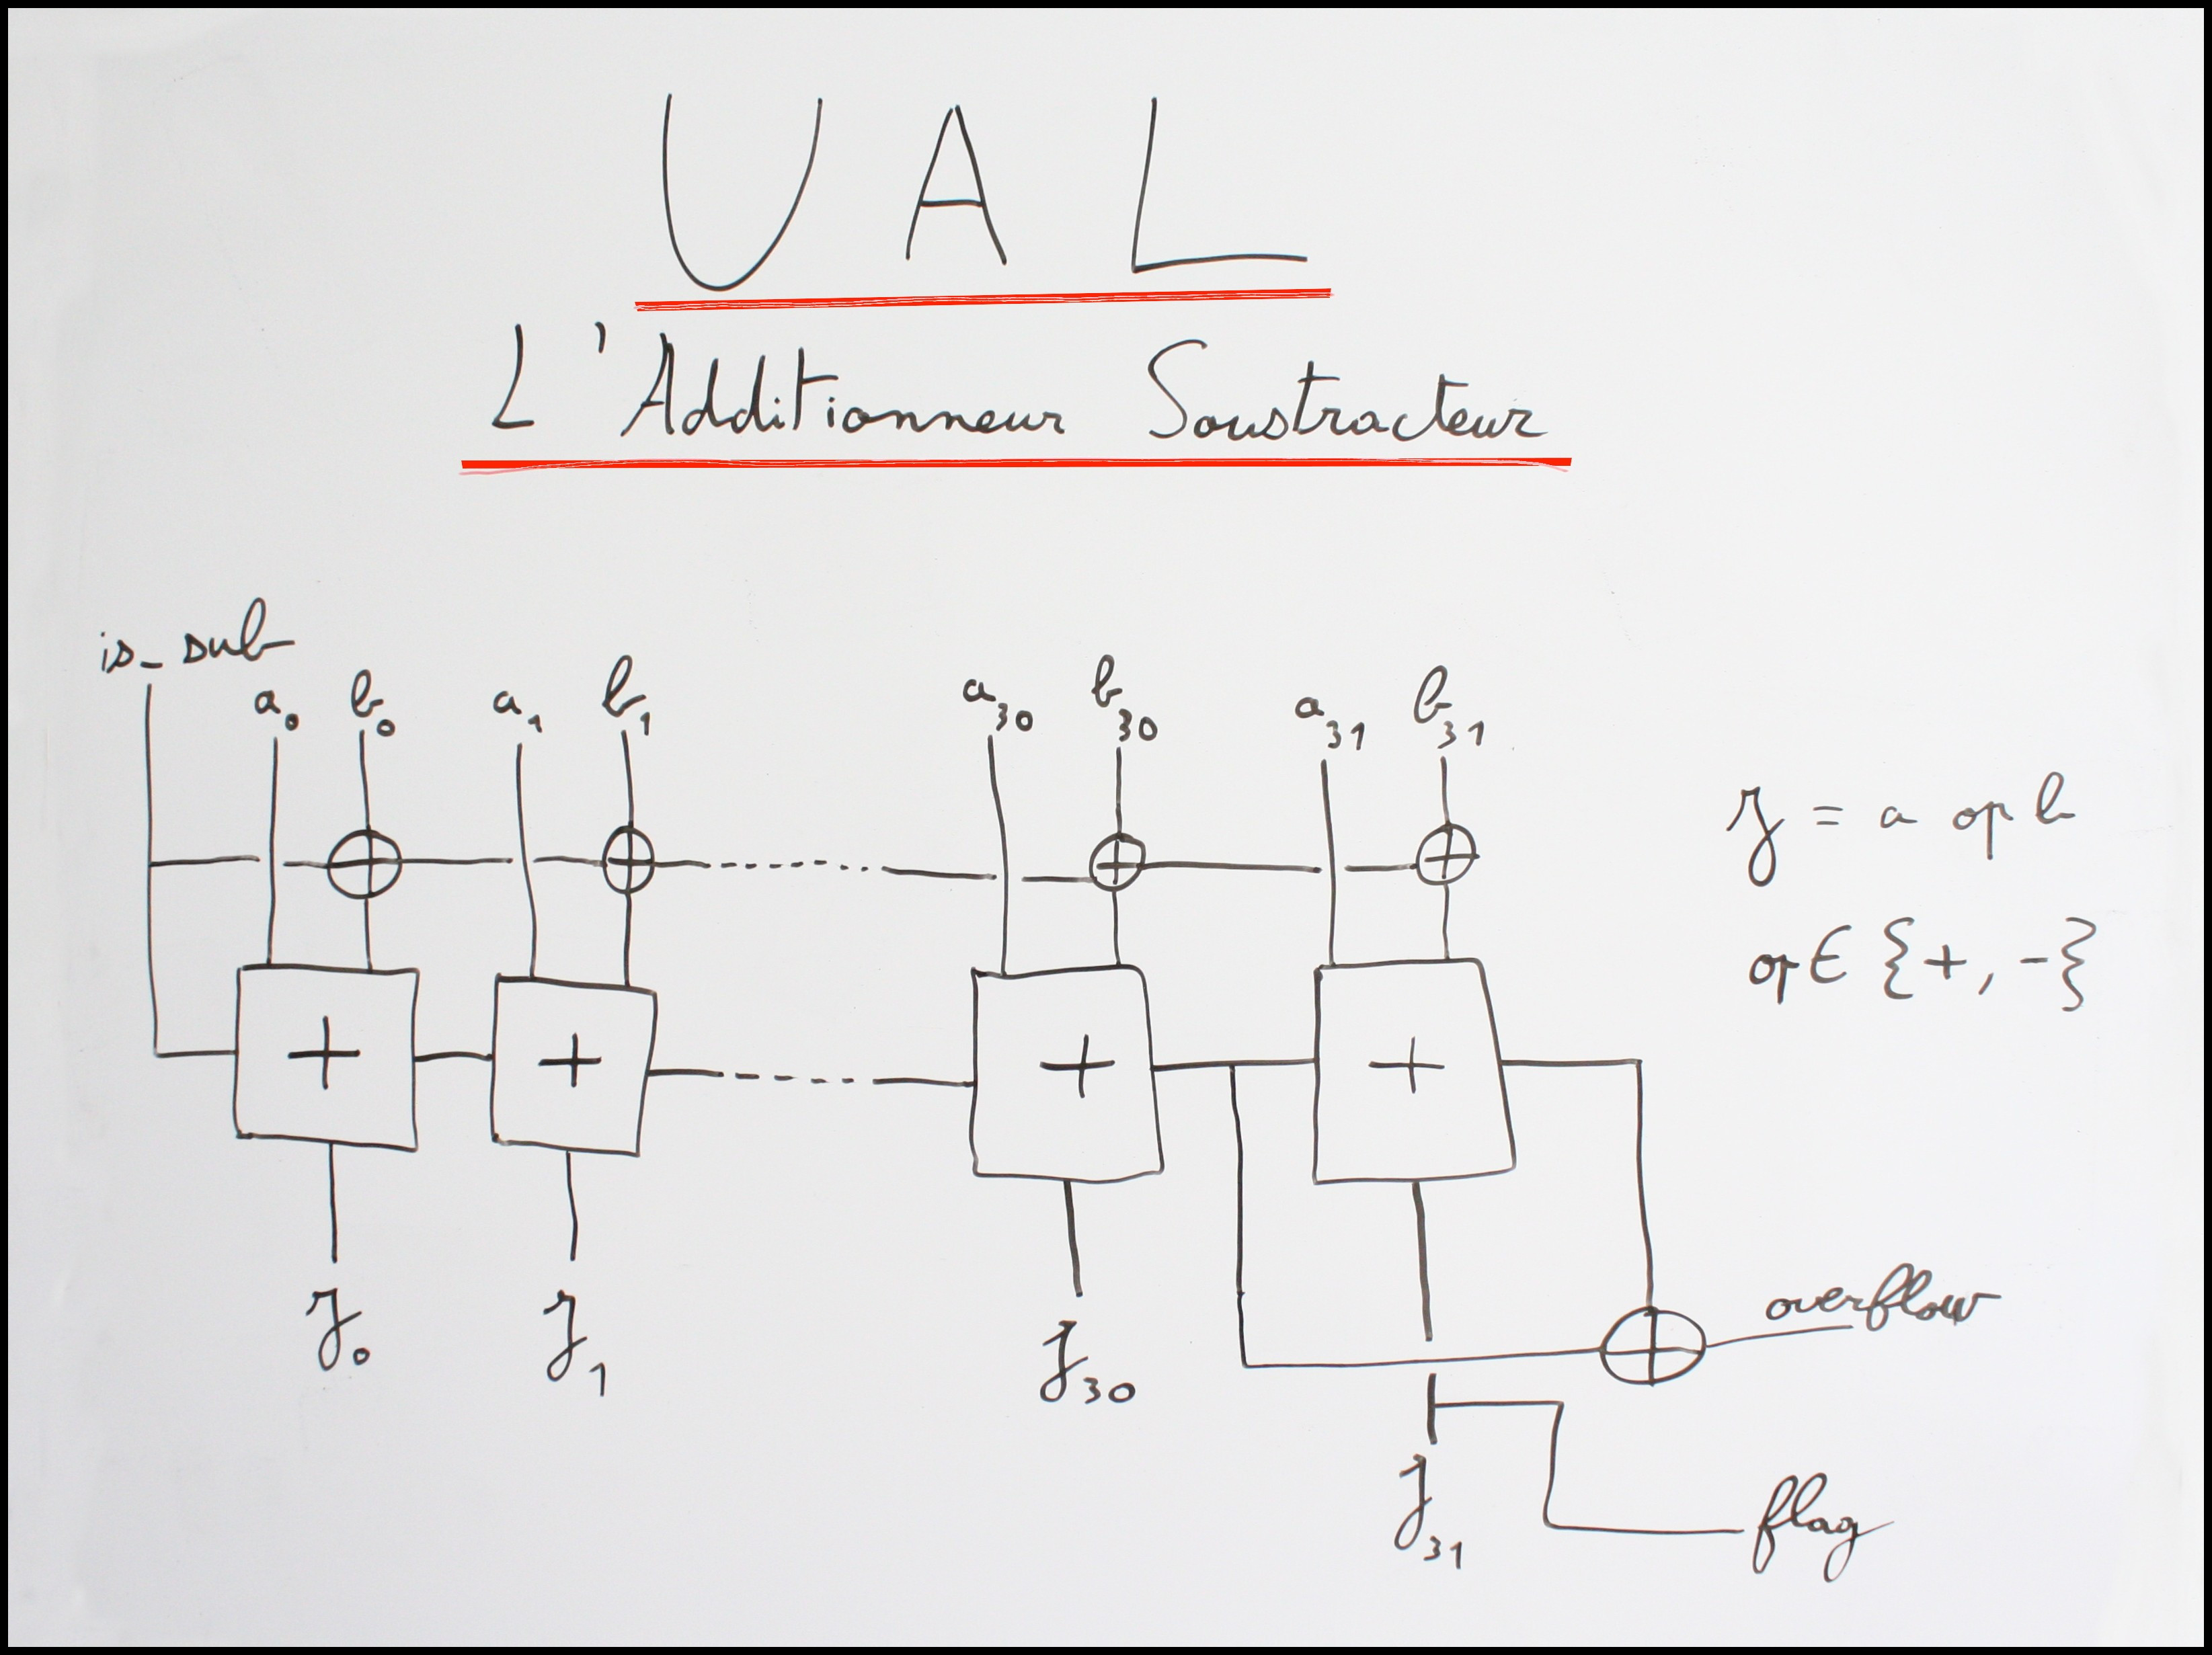
\includegraphics[width=10cm]{additionneur.jpg}
%\caption{Cryptage Asymétrique}
\end{figure}

\subsection{Les instructions matérielles}

Les instructions du microprocesseur sont codé sur 27 bits. Les 4 premiers bits 
codent l'instruction voulue. Le reste du codage l'instruction dépend de sa nature.
Si la description du codage d'une instruction ne va pas jusqu'à 27 bits (notamment
quand il n'y a pas d'argument entier), il est sous entendu que le code de 
l'instruction est complété par des zéros à la fin.

Le microprocesseur supporte les 12 instructions suivantes.

\subsubsection{ADD(i)}

L'instruction ADD implémente l'addition. Elle s'emploie de la façon suivante :
ADD a b. Cette instruction calcule la somme des valeurs contenues dans les mémoires
a et b, et place le résultat dans la mémoire b.\\
L'instruction supporte que sont premier paramètre soit directement un nombre, l'addition
s'effectue alors directement avec celui-ci.\\

Le code de l'instruction prend la forme suivante :

\begin{tabular}{|c|c|c|c|}
  \hline
  0000 & 0 & premier registre (a) & second registre (b) \\
  \hline
\end{tabular}\\

Dans le cas ou le premier argument est directement un entier (instruction ADDi),
le code de l'instruction prend cette forme :

\begin{tabular}{|c|c|c|c|}
  \hline
  0000 & 1 & entier (sur 16 bits) & registre (b) \\
  \hline
\end{tabular}\\

\subsubsection{SUB(i)}

L'instruction SUB implémente la soustraction. Elle s'emploie de la façon suivante :
SUB a b. Cette instruction calcule la différence des valeurs contenues dans les mémoires
a et b (b - a), et place le résultat dans la mémoire b.\\
L'instruction supporte que sont premier paramètre soit directement un nombre, la soustraction
s'effectue alors directement avec celui-ci.\\

Le code de l'instruction prend la forme suivante :

\begin{tabular}{|c|c|c|c|}
  \hline
  0001 & 0 & premier registre (a) & second registre (b) \\
  \hline
\end{tabular}\\

Dans le cas ou le premier argument est directement un entier (instruction SUBi),
le code de l'instruction prend cette forme :

\begin{tabular}{|c|c|c|c|}
  \hline
  0001 & 1 & entier (sur 16 bits) & registre (b) \\
  \hline
\end{tabular}\\

\subsubsection{MOVE(i)}

L'instruction MOVE implémente la copie d'octet


\subsubsection{AND}

L'instruction AND implémente un "et" logique bit à bit. Elle s'emploie de la façon suivante :
ADD a b. Cette instruction calcule le "et" logique entre les bits de la mémoire de a et b, 
et place le résultat dans la mémoire b.\\

Le code de l'instruction prend la forme suivante :

\begin{tabular}{|c|c|c|c|}
  \hline
  0011 & 0 & premier registre (a) & second registre (b) \\
  \hline
\end{tabular}\\

\subsubsection{OR}

L'instruction OR implémente un "ou" logique bit à bit. Elle s'emploie de la façon suivante :
OR a b. Cette instruction calcule le "ou" logique entre les bits de la mémoire de a et b, 
et place le résultat dans la mémoire b.\\

Le code de l'instruction prend la forme suivante :

\begin{tabular}{|c|c|c|c|}
  \hline
  0100 & 0 & premier registre (a) & second registre (b) \\
  \hline
\end{tabular}\\

\subsubsection{XOR}

L'instruction XOR implémente un "ou exclusif" logique bit à bit. Elle s'emploie de la façon suivante :
XOR a b. Cette instruction calcule le "ou exclusif" logique entre les bits de la mémoire de a et b, 
et place le résultat dans la mémoire b.\\

Le code de l'instruction prend la forme suivante :

\begin{tabular}{|c|c|c|c|}
  \hline
  0101 & 0 & premier registre (a) & second registre (b) \\
  \hline
\end{tabular}\\

\subsubsection{NOT}

L'instruction NOT implémente un "non" logique bit à bit. Elle s'emploie de la façon suivante :
NOT a b. Cette instruction calcule le "non" logique des bits de la mémoire de a,
et place le résultat dans la mémoire b.\\

Le code de l'instruction prend la forme suivante :

\begin{tabular}{|c|c|c|c|}
  \hline
  0110 & 0 & premier registre (a) & second registre (b) \\
  \hline
\end{tabular}\\

\subsubsection{LSE}

L'instruction LSE implémente un décalage de un bit à gauche. Elle s'emploie de la façon suivante :
LSE a. Cette instruction décale les bits à gauche de la mémoire de a, et place le résultat dans la mémoire a.\\

Le code de l'instruction prend la forme suivante :

\begin{tabular}{|c|c|c|}
  \hline
  0111 & 0 & registre (a) \\
  \hline
\end{tabular}\\

\subsubsection{RSE}

L'instruction RSE implémente un décalage de un bit à droite. Elle s'emploie de la façon suivante :
RSE a. Cette instruction décale les bits de la mémoire à droite de a, et place le résultat dans la mémoire a.\\

Le code de l'instruction prend la forme suivante :

\begin{tabular}{|c|c|c|}
  \hline
  1000 & 0 & registre (a) \\
  \hline
\end{tabular}\\

\subsubsection{EQZ(i)}

L'instruction EQZ implémente un saut conditionnel si le flag indique une égalité à zéro. 
Elle s'emploie de la façon suivante : EQZ a. Si le flag indique une égalité à zéro, 
cette instruction incrémente le pointeur d'instruction de la valeur contenue dans 
la mémoire a.\\
L'instruction supporte que sont premier paramètre soit directement un nombre, la saut
s'effectue alors directement avec celui-ci.\\

Le code de l'instruction prend la forme suivante :

\begin{tabular}{|c|c|c|}
  \hline
  1001 & 0 & registre (a) \\
  \hline
\end{tabular}\\

Dans le cas ou le premier argument est directement un entier (instruction EQZi),
le code de l'instruction prend cette forme :

\begin{tabular}{|c|c|c|}
  \hline
  1001 & 1 & entier (sur 16 bits)\\
  \hline
\end{tabular}\\

\subsubsection{LTZ(i)}

L'instruction LTZ implémente un saut conditionnel si le flag indique une infériorité à zéro. 
Elle s'emploie de la façon suivante : LTZ a. Si le flag indique une infériorité à zéro, 
cette instruction incrémente le pointeur d'instruction de la valeur contenue dans 
la mémoire a.\\
L'instruction supporte que sont premier paramètre soit directement un nombre, la saut
s'effectue alors directement avec celui-ci.\\

Le code de l'instruction prend la forme suivante :

\begin{tabular}{|c|c|c|}
  \hline
  1010 & 0 & registre (a) \\
  \hline
\end{tabular}\\

Dans le cas ou le premier argument est directement un entier (instruction LTZi),
le code de l'instruction prend cette forme :

\begin{tabular}{|c|c|c|}
  \hline
  1010 & 1 & entier (sur 16 bits)\\
  \hline
\end{tabular}\\

\subsubsection{MTZ(i)}

L'instruction MTZ implémente un saut conditionnel si le flag indique une supériorité à zéro. 
Elle s'emploie de la façon suivante : MTZ a. Si le flag indique une supériorité à zéro, 
cette instruction incrémente le pointeur d'instruction de la valeur contenue dans 
la mémoire a.\\
L'instruction supporte que sont premier paramètre soit directement un nombre, la saut
s'effectue alors directement avec celui-ci.\\

Le code de l'instruction prend la forme suivante :

\begin{tabular}{|c|c|c|}
  \hline
  1011 & 0 & registre (a) \\
  \hline
\end{tabular}\\

Dans le cas ou le premier argument est directement un entier (instruction MTZi),
le code de l'instruction prend cette forme :

\begin{tabular}{|c|c|c|}
  \hline
  1011 & 1 & entier (sur 16 bits)\\
  \hline
\end{tabular}\\

\newpage~

\subsection{Les macros}

De ces instructions de bases implémentées en matériel, on pourra écrire des macros pour 
des fonctions de plus haut niveau. Le multiplier peut par exemple se réaliser à coup 
d'additions et de sauts conditionnels (on suppose ici que les deux facteurs se trouvent 
dans les registres r2 et r3, le résultat sera stocké dans r1) :\\

\begin{lstlisting}
XOR r1 r1 // Mise a zero du registre de retour
ADD 0 r3  // Initialise le flag qui va permettre de savoir si r3 = 0
EQZ 4     // Si r3 est egal a 3, on ne fait rien, on saute
ADD r2 r1 // Sinon on additionne et on decremente
SUB 1 r3
EQZ -2    // On teste l'egalite a 0, s'il n'est pas encore a 0 on recommence !
\end{lstlisting}




\newpage~

\section*{Conclusion}
\addcontentsline{toc}{section}{Conclusion}

\end{document}


